\documentclass[20pt]{ctexart}
\usepackage{graphicx}
\usepackage{amsmath}
\usepackage{url}
\usepackage{subfigure}
\usepackage{float}
\usepackage{lmodern}
\usepackage{xeCJK}
\usepackage{tikz}
\usepackage{enumitem}
\usepackage{verbatimbox}
\usepackage{cite}
\usepackage{amsfonts}
\usepackage{amsthm}
\usepackage{geometry}
\usepackage{verbatimbox}
\usepackage{caption}
\usepackage{listings}
\usepackage[ruled,linesnumbered]{algorithm2e}

%设置新环境
\newtheorem{example}{例}             
\newtheorem{theorem}{定理}[section] 
\newtheorem{definition}{定义}[section]
\newtheorem{property}{性质}
\newtheorem{proposition}{命题}
\newtheorem{lemma}{引理}
\newtheorem{corollary}{推论}
\newtheorem{remark}{注}
\newtheorem{condition}{条件}
\newtheorem{conclusion}{结论}
\newtheorem{assumption}{假设}
\newenvironment{solution}{\begin{proof}[\indent\bf 解]}{\end{proof}}%设置新环境
\CTEXsetup[format={\Large\bfseries}]{section}%加入字体
\geometry{a4paper,scale=0.8}%设置文档格式
\tikzstyle{file} = [rectangle, rounded corners, minimum width = 3cm, minimum height=1.2cm ,text centered, draw = black]%设置流程图
\tikzstyle{dots} = [rectangle, rounded corners, minimum width = 1.5cm, minimum height=2cm ,text centered, draw = black,text width=3cm]%设置流程图
\tikzstyle{arrow} = [->,>=stealth]%设置流程图
\usetikzlibrary{arrows, decorations.pathmorphing, backgrounds, positioning, fit, petri, automata}%使用流程图元素
\bibliographystyle{unsrt}%设置引用格式

\title{Lab2 Report}
\author{作者:罗文杰\\专业: 计算机科学与技术\\学号: 3210102456}
\date{}

\begin{document}
\maketitle

\section{Introduction}
In this lab, we will write a program to convert numbers to hexadecimal.

\section{construst}
The construsts of the program is as follows.

\begin{center}
    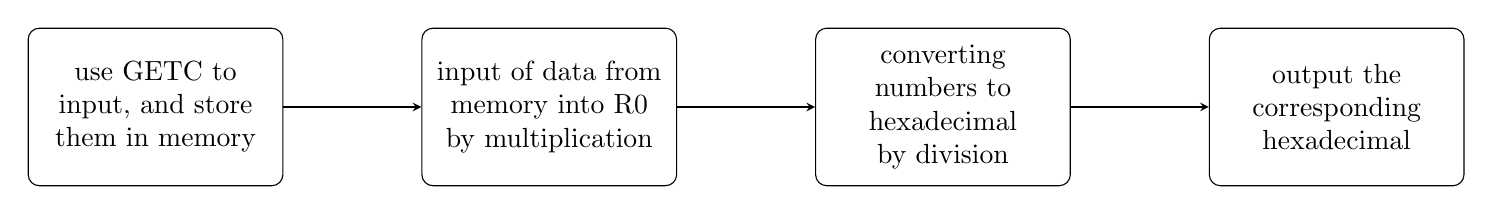
\begin{tikzpicture}[node distance = 2.5cm]
      \node[dots] (in) at (-7.5,0) {use GETC to input, and store them in memory};
      \node[dots] (set1) at (-2.5,0){input of data from memory into R0 by multiplication};
      \node[dots] (set2) at (2.5,0){converting numbers to hexadecimal by division};
      \node[dots] (out1) at (7.5,0){output the corresponding hexadecimal};
    
      \draw[arrow](in) -- node[anchor=east,xshift=0.75cm,yshift=0.3cm]{}(set1);
      \draw[arrow](set1) -- node[anchor=east,xshift=0.8cm,yshift=0.3cm]{}(set2);
      \draw[arrow](set2) -- node[anchor=east,xshift=0.6cm,yshift=0.5cm] {}(out1);
    \end{tikzpicture}
    \end{center}

\section{Improvment}
There are two points to improve.

\subsection{fast multiplication}
First, in step 2, we need use multiplication to take numbers from memory into R0, and it needs cumulative addition to realize multiplication convincing that the input numbers may have many bits. And Repeated addition is too time consuming, so we need to use fast multiplication to achieveit.

When multiplying a number X with some constant, we can decompose the constant into a number of numbers that add up to a base of two, and then multiply X with each of these numbers and add them again. This algorithm reduces the number of operations because X can be multiplied with $2^k$ by having X shifted left by k bits to achieve this.

In this program, 10 = 2 + 8, so we can have R0 shifted one place left to add to the number shifted 3 places left. This algorithm requires only 4 operations, which is a significant improvement over the original 10.

The codes is as follows.
\begin{verbatim}
    ;The CHAR1 already had the input
    DONE    AND R0, R0, #0 ; binary num
            LEA R3, CHAR1
    LOOP    LDR R1, R3, #0
            ADD R3, R3, #1
            ADD R0, R0, R1
            ADD R2, R2, #-1
            BRz LOOPUOT
            ADD R1, R0, R0 ; shift 1 place
            ADD R0, R1, R1 ; shift 2 places
            ADD R4, R0, R0 ; shift 3 places
            ADD R0, R4, R1 ; R0 = 2 * R0 + 8 * R0
            BRnzp LOOP
    ; R0 has the number
\end{verbatim}

\subsection{right shift}
Second, in step 3, we need to use addition to achieve the division operation, but this is too time consuming.

To cover this problems, we have another solution: Let the data in R0 be cyclically shifted to the right, each time by 4 bits and then let the result be an iso-or operation with x000F to store the result in memory.

However, there is no right shift instruction in LC-3 and we need to use a left shift instead of a right shift. Before each left shift, identify the first position of the data in R0, if it is 1, the result will be added by 1 after the left shift, otherwise it will be shifted directly left without adding 1.

The codes is as follow.

\begin{verbatim}
    LOOPUOT LEA R3, MARK ; output char addressing -1
            ADD R2, R2, #5 ; counter
            AND R5, R5, #0
            LD  R4, PDIV ; mask
    ; bigin to trans
    TRANS   ADD R5, R5, #4
            AND R1, R0, R4
            STR R1, R3, #0
            ADD R3, R3, #1
            ADD R2, R2, #-1
            BRz OUTPUT
    RIGHT   ADD R0, R0, #0
            BRzp ZARO
            BRnzp ONE
    ZARO    ADD R0, R0, R0
            BRnzp ALOOP
    ONE     ADD R0, R0, R0
            ADD R0, R0, #1
    ALOOP   ADD R5, R5, #-1
            BRz TRANS
            BRnzp RIGHT
    ; output
\end{verbatim}

\end{document}
